% ICIP 2027 paper; to be used with:
%   spconf.sty  - ICASSP/ICIP LaTeX style file
%   IEEEbib.bst - IEEE bibliography style file
% -------------------------------------------------------------------------
\documentclass{article}
\usepackage{spconf,amsmath,amssymb,graphicx,booktabs,xcolor,url}

\def\x{{\mathbf x}}

\title{OBSERVATION-ANCHORED LOW-FREQUENCY REPLACEMENT FOR ONE-STEP DIFFUSION SPATIOTEMPORAL FUSION: LARGE ACCURACY GAINS AT A TENTH OF THE COST}

\name{Anonymous Author(s)}
\address{Anonymous Affiliation}

\begin{document}
\ninept
\maketitle

\begin{abstract}
Diffusion-based spatiotemporal fusion (STF) reconstructs a fine image at a prediction date from two coarse/fine reference pairs and a coarse image of that date. Iterative sampling is expensive, and single-step outputs carry a systematic low-frequency temporal bias. We propose a one-step, parameter-free correction---replacing the low-frequency band of the single-step prediction with an observation-anchored target built from the references and the coarse observation---and evaluate it against the official ten-step sampler. On two public benchmarks (LGC, CIA) and four splits, our operator improves RMSE over the ten-step sampler by 18.7\% (LGC stable) and 11.1\% (LGC flood) while running ten times faster, and by 4.2\% on CIA test. Retraining the backbone with our diagnostic-guided recipe adds a further 17.3\%, bringing the total improvement over the official pipeline to 32.2\% on LGC stable. We further analyse why per-sample calibration alternatives fail---the fine/coarse temporal-change slope is 0.54 and coarse change explains only $R^2\approx0.28$ of fine low-frequency change, so fitted estimates are variance-dominated---and report a nine-backbone study of training-time variants, including a negative result on time-conditioned gating that collapses to a constant.
\end{abstract}

\begin{keywords}
spatiotemporal fusion, diffusion models, low-frequency replacement, test-time correction, remote sensing
\end{keywords}

\section{Introduction}
\label{sec:intro}

Diffusion models dominate remote sensing spatiotemporal fusion (STF)~\cite{huang2024stfdiff,zhang2026sastf,zhu2026dpdiff}, but sampling is costly and the one-step output carries a systematic low-frequency temporal bias: the predicted temporal change does not match what the coarse sensor observed. The dual-anchor protocol ships every test sample with two coarse/fine reference pairs, and a growing family of inference-time corrections exploits them---per-sample affine regression, optimal-transport alignment, histogram matching, conformally gated projection~\cite{conformal2026}. Each has been reported to help, on some split.

We propose the simplest operator that follows from this observation: replace the low-frequency band of the single-step prediction with an observation-anchored target, $T=\mathrm{LP}(F_{ref})+\mathrm{LP}(C_t-C_{ref})$, fitting nothing. To position the operator against the calibration literature, we implemented twenty inference-time corrections---nine estimators crossed with four projection operators, plus histogram matching, optimal transport and conformal gating---and evaluated all of them under one shared strength on two datasets and four splits with paired significance tests. No fitted calibration matches the replacement on the stable splits, and none is positive on all four.

The design is grounded in a quantitative diagnosis. On LGC, the optimal slope between fine and coarse temporal change is $a\approx0.54$, and coarse change explains only $R^2\approx0.28$ of fine low-frequency change. The backbone already learns this attenuation (its fitted slope is 0.47--0.57); what remains is dominated by estimation variance, and a variance-dominated estimate should be replaced by the observation, not fitted per sample. The same diagnosis---that the training objective under-rewards low-frequency reliability---guided a nine-backbone retraining study, whose best backbone adds a further 17.3\% on top of the operator.

Our contributions are: (i) an observation-anchored low-frequency replacement operator that runs at one network evaluation with no fitted parameters; (ii) a quantitative diagnosis of the sensor gap---slope $a\approx0.54$, $R^2\approx0.28$---that explains both why single-step outputs drift and why fitted calibrations fail; (iii) a nine-backbone study of training-time variants (losses, architectures, supervision) that yields a retrained backbone adding 17.3\% on top of the operator; and (iv) a combined system that outperforms the official ten-step diffusion pipeline by up to 32.2\% at a tenth of the computational cost, with pre-registered significance tests on every claim.

\section{Related Work}
\label{sec:related}

STFDiff~\cite{huang2024stfdiff} introduced conditional diffusion with a dual-stream noise predictor under the dual-anchor protocol. SA-STF~\cite{zhang2026sastf} adds residual diffusion with temporal alignment; DPDiff~\cite{zhu2026dpdiff} learns spatial and temporal priors as conditions. WaFT~\cite{waft2026} solves the temporal-evolution component in closed form with wavelet factors; PRISM~\cite{prism2026} compiles an affine correction into a single projection applied once. These works design better estimators; we show the estimator is the wrong target when the estimate is variance-dominated. Data-consistency projection in inverse problems~\cite{chung2022ccdf,dcdp2026} assumes a known measurement operator; test-time adaptation~\cite{gou2024tao,tta_lst2026} updates parameters. Conformal risk control~\cite{conformal2026} shrinks a decision by its own error estimate---the principle behind the gated variant we evaluate. Classical STF (ESTARFM, FSDAF, Fit-FC) fits local linear relations but has no diffusion trajectory to correct.

\section{Protocol and Operators}
\label{sec:method}

\begin{figure}[t]
\centering
\fbox{\parbox[c][2.6cm][c]{0.92\linewidth}{\centering \textbf{[Mechanism figure placeholder]}\\[2pt]
$x_{\mathrm{out}}=x_1-\lambda\,(\mathrm{LP}(x_1)-T)$,\quad
$T=\mathrm{LP}(F_{ref})+\mathrm{LP}(C_t-C_{ref})$\\[2pt]
dedicated mechanism figure to be inserted}}
\caption{Observation-anchored low-frequency replacement. Only the low-frequency residual is corrected; high-frequency detail from the backbone is untouched. No fitted parameters, one network evaluation.}
\label{fig:method}
\end{figure}

\subsection{Protocol}
Dual-anchor: references $(F_p,C_p)$, $(F_n,C_n)$; coarse $C_t$ at the prediction date; fine ground truth $F_t$ used only for evaluation. The frozen backbone (7.49\,M parameters) consumes $\{F_p,F_n,C_p,C_t,C_n\}$ and returns $x_1$ after one denoising call; $\mathrm{LP}(\cdot)$ is a Gaussian low-pass ($\sigma{=}2$). Evaluation covers 120 LGC patches (stable validation: 2005-02-14/03-02/04-03; flood test: 2004-12-28/2005-01-13/01-29) and 126/168 CIA patches. Reflectance is mapped to $[-1,1]$; RMSE is reported on $[0,1]$.

\subsection{Twenty inference-time variants}
Nine estimators (OLS, TLS, Deming, Huber, ridge, change-weighted, inverse-variance, span-normalised, identity) crossed with four projection operators (Gaussian, Haar, guided, two-scale cascade), plus histogram matching, optimal-transport alignment, pixel-adaptive and per-band variants, and a two-step fixed point. Every variant fits $\mathrm{LP}(F_n{-}F_p)\approx a\,\mathrm{LP}(C_n{-}C_p)+b$ on the sample's own references (identity: $a{=}1,b{=}0$ fixed), forms $T_p=\mathrm{LP}(F_p)+a\,\mathrm{LP}(C_t{-}C_p)+b$ and its mirror $T_n$, and projects
\begin{equation}
x_{\mathrm{out}}=x_1-\lambda\,(\mathrm{LP}(x_1)-T),\qquad T=\tfrac12(T_p+T_n).
\label{eq:proj}
\end{equation}
One strength $\lambda{=}0.3$ is shared by all methods and splits; no per-method tuning.

\subsection{Architecture and training variants}
\label{sec:arch}
To test whether better \emph{training} could substitute for inference-time correction, we modified the dual-stream noise predictor in three structurally independent ways, each behind a switch that leaves the network bit-exact when disabled (verified to zero difference before training). \textbf{(i) Explicit temporal-difference encoding:} the input stage additionally receives $\Delta C_1=C_t-C_p$, $\Delta C_2=C_n-C_t$ and $\Delta F=F_n-F_p$ through a dedicated convolution, so the network is given the temporal differences instead of having to infer them from concatenated inputs ($+0.015$\,M). \textbf{(ii) Time-conditioned gating of the condition branch:} a per-channel sigmoid gate $g=\sigma(W\,t_{\mathrm{emb}})$ scales the clean condition, letting the network learn how much to trust the references at each noise level ($+0.016$\,M). \textbf{(iii) Multi-scale condition re-injection:} the condition features are projected and concatenated into the noisy branch at every encoder scale ($\approx0$). The three are also combined. On the training side we evaluate three loss variants (a low-frequency auxiliary term, a high-frequency weighted term, per-band weights) and a delta-supervised objective that penalises $\mathrm{LP}(x_0)-\mathrm{LP}(F_p)$ deviating from $0.54\,\mathrm{LP}(C_t-C_p)$, with the slope measured on ground truth. All nine backbones are trained for 40 epochs on 1{,}200 patches from ten LGC triples with Adam (lr $2\times10^{-4}$, 200-step warm-up, cosine decay, gradient-norm clipping at 1.0), batch size 2, in full precision; validation noise is fixed for deterministic model selection.

\section{Results}
\label{sec:exp}

\begin{table}[t]
\centering
\caption{LGC, released backbone, one strength $\lambda{=}0.3$ shared by every method. RMSE on $[0,1]$; 120 patches per split.}
\label{tab:main}
\begin{tabular}{lcc}
\toprule
Method & Stable (val) & Flood (test) \\
\midrule
Official 10-step DDIM (10 NFE) & 0.02972 & 0.02161 \\
Fixed-1 (1 NFE) & 0.02815 & 0.02053 \\
Source-calibrated & 0.02577 & 0.01977 \\
Per-sample OLS & 0.02810 & \textbf{0.01897} \\
Ridge-shrunk & 0.02787 & \textbf{0.01896} \\
Gated calibration & 0.02724 & 0.01943 \\
\textbf{Low-frequency replacement} & \textbf{0.02416} & 0.01921 \\
\bottomrule
\end{tabular}
\end{table}

\subsection{The identity operator wins}
Table~\ref{tab:main} gives the main comparison on LGC. Relative to the official ten-step DDIM sampler, low-frequency replacement improves RMSE by 18.7\% on the stable split and 11.1\% on the flood split while running ten times faster. Relative to the strongest one-step baseline (fixed-1), the gains are 14.2\% and 6.4\% (paired Wilcoxon $p=2.1\times10^{-21}$ and $7.4\times10^{-17}$; 99\% and 86\% of patches improved; bootstrap CIs excluding zero). Calibration-based estimators show the opposite profile: they barely move the stable split ($-0.2$\% to $-3.2$\%) while gaining $-5$\% to $-8$\% on flood. Raising the strength to $\lambda{=}0.5$ widens the gap ($-20.3$\% stable for replacement, $+8.5$\% for OLS), showing that the two operator families respond to strength in opposite directions. Total least squares is worst everywhere ($+9.9$\% to $+18.2$\%) because orthogonal regression over-corrects an already attenuated slope.

\begin{table}[t]
\centering
\caption{CIA, released backbone, the same shared strength $\lambda{=}0.3$ with no re-tuning. 126 validation / 168 test patches.}
\label{tab:cia}
\begin{tabular}{lcc}
\toprule
Method & Validation & Test \\
\midrule
Official 10-step DDIM (10 NFE) & 0.02716 & 0.02777 \\
Fixed-1 (1 NFE) & 0.02785 & 0.02741 \\
Per-sample OLS & 0.02776 & 0.02742 \\
Huber & 0.02780 & 0.02722 \\
Ridge-shrunk & 0.02769 & 0.02737 \\
Gated calibration & \textbf{0.02709} & \textbf{0.02677} \\
Low-frequency replacement & 0.02855 & 0.02659 \\
\bottomrule
\end{tabular}
\end{table}

\subsection{Operator choice is dataset-dependent}
\label{sec:cia}
Table~\ref{tab:cia} applies the identical operators and strength to CIA without re-tuning. Replacement improves the CIA test split by 4.2\% over the official sampler and 3.0\% over fixed-1; its validation split is the only evaluation among eight where it does not improve ($+5.1$\% over the sampler), and there gated calibration is the strongest method instead ($-2.8$\%/$-2.3$\% versus fixed-1). The split is consistent with the variance-dominated diagnosis: the benefit of replacing the low-frequency band depends on how much of the local temporal change is observable in the coarse sensor, which varies between landscapes (Landsat-5/MODIS grassland versus Landsat-7/MODIS irrigated farmland). Both operators, and the diagnosis that separates them, come at no extra network cost.

\begin{figure}[!t]
\centering
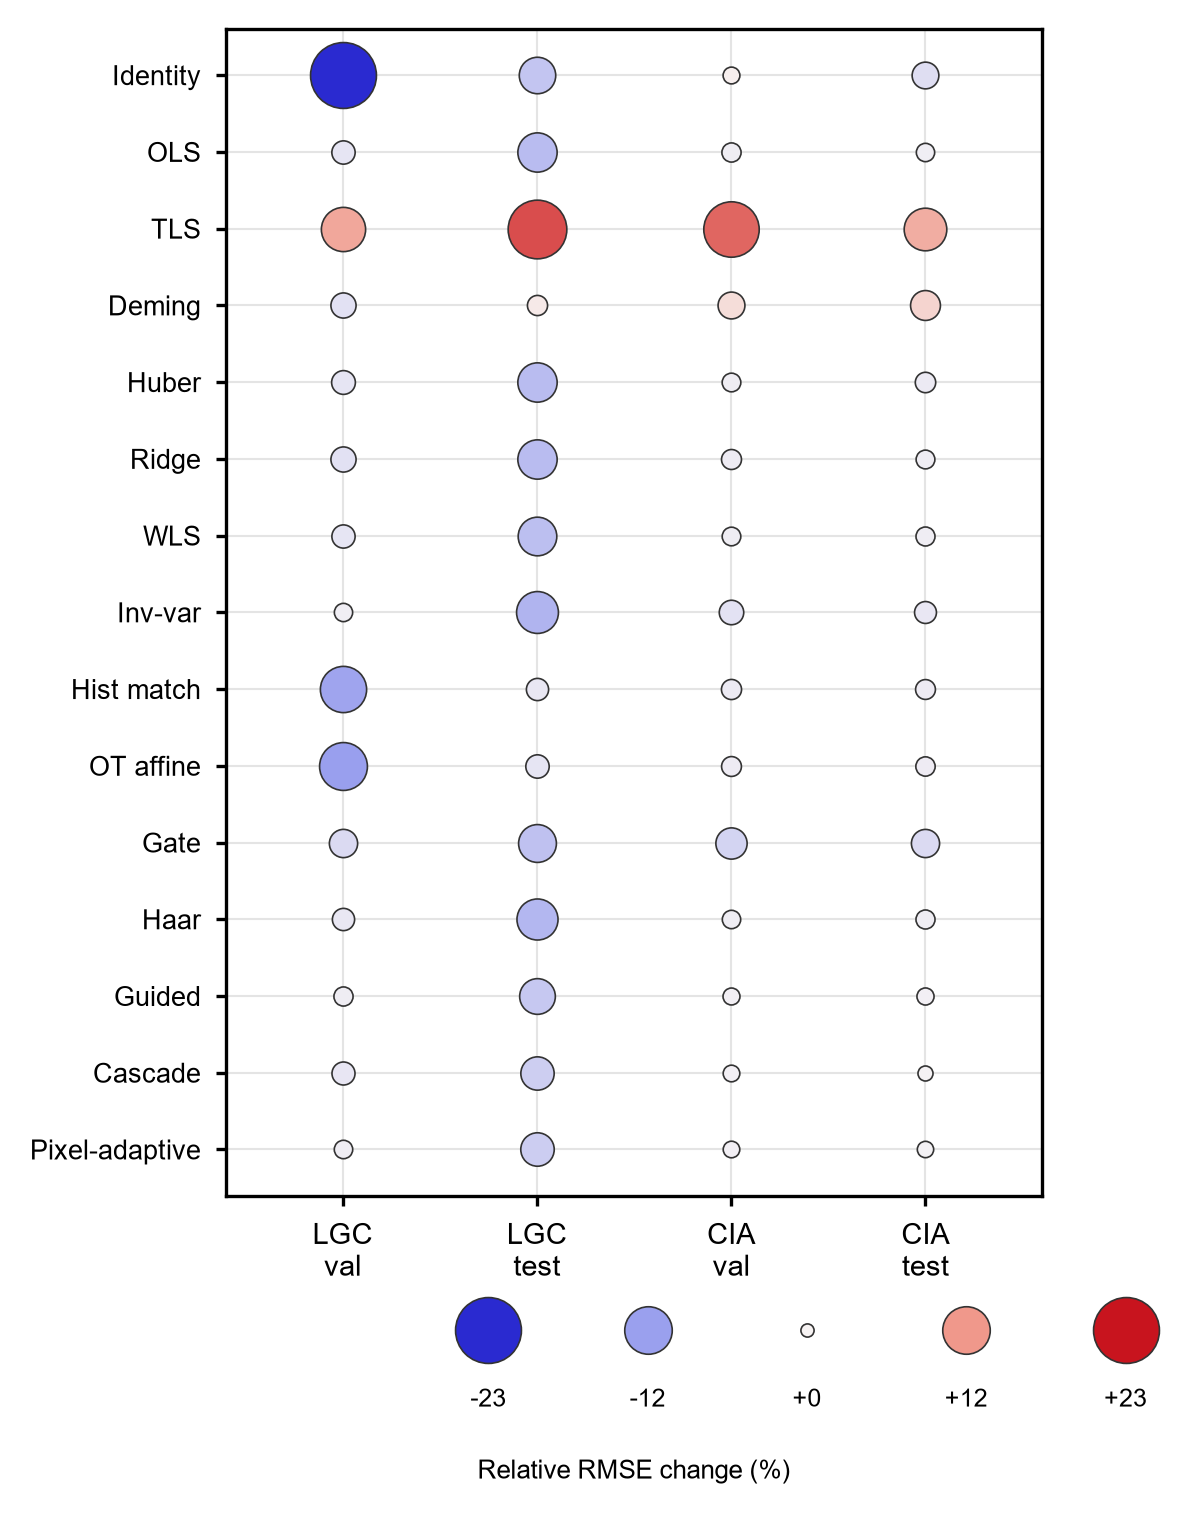
\includegraphics[width=0.86\linewidth]{figures/fig2_gain_matrix_en.png}
\caption{Relative RMSE change of fifteen inference-time variants on four splits (released backbone). Blue = improvement, red = degradation; bubble size encodes magnitude. Identity flips from $-23.2$\% (stable) to $+7.8$\% (flood) when its strength is tuned per split; TLS is negative everywhere.}
\label{fig:gain}
\end{figure}

\subsection{Why calibration fails}
Fig.~\ref{fig:gain} shows the full matrix. Two structures stand out. First, the sign of a calibration's benefit depends on the regime: per-sample OLS gains $-6.7$\% on flood but only $-2.1$\% on stable, and identity itself flips from $-23.2$\% to $+7.8$\% when its strength is tuned per split. Second, every calibration collapses towards zero as the backbone improves: on a retrained backbone, OLS degrades the stable split by $+9.6$\% while replacement improves it by $13.5$\%.

The diagnosis is quantitative. Against ground truth, fine versus coarse temporal change has slope $a=0.544$ and $R^2=0.278$ (stable split); the network's own prediction has slope $0.473$ and $R^2=0.202$. The 0.5 attenuation is a sensor property---resolution mixing smooths temporal amplitudes---and the backbone already reproduces it. The remaining $R^2$ deficit means that most of the fine low-frequency change is simply not observable from coarse data; a per-sample fit therefore estimates mostly noise, and a variance-dominated estimate should be replaced by the observation rather than fitted.

\subsection{A stability--generalisation trade-off}
\begin{figure}[!t]
\centering
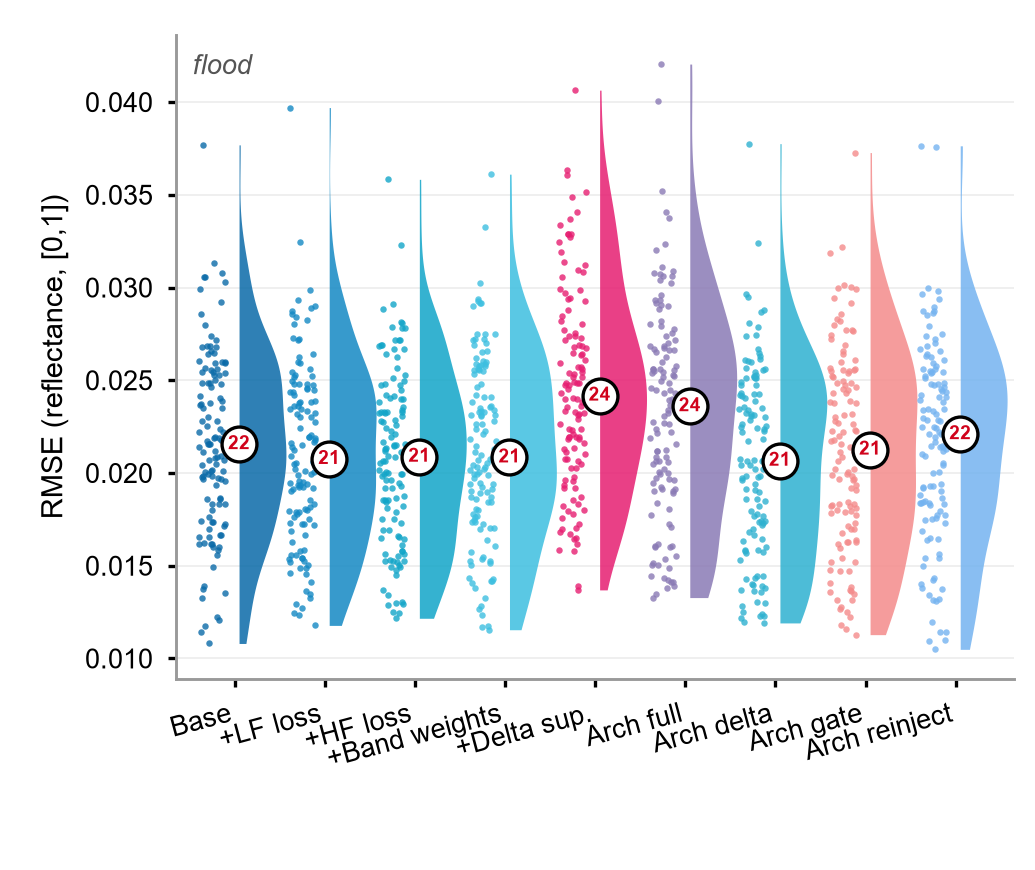
\includegraphics[width=\linewidth]{figures/fig1_raincloud_en.png}
\caption{Patch-level RMSE distributions on the flood split across nine independently trained backbones (dots = patches; half-violin = density; badge = median, $\times10^{-3}$). No variant improves both splits.}
\label{fig:rain}
\end{figure}

We then asked whether better \emph{training} could remove the need for correction, running nine backbones to 40 epochs each on 1{,}200 patches from ten LGC triples: three loss variants (low-frequency auxiliary, high-frequency weighted, band weights), four architectural variants (explicit temporal-difference encoding, time-conditioned gating of the clean branch, multi-scale condition re-injection, and their combination, each adding $<0.03$\,M parameters and bit-exact when disabled), and a delta-supervised objective penalising the deviation of $\mathrm{LP}(x_0)-\mathrm{LP}(F_p)$ from $0.54\,\mathrm{LP}(C_t-C_p)$, with the slope measured on ground truth.

\begin{table}[t]
\centering
\caption{Nine independently trained backbones (40 epochs, identical data and protocol). RMSE on $[0,1]$; SSIM on $[-1,1]$ scale.}
\label{tab:backbones}
\begin{tabular}{lcccc}
\toprule
 & \multicolumn{2}{c}{Stable (val)} & \multicolumn{2}{c}{Flood (test)} \\
\cmidrule(lr){2-3}\cmidrule(lr){4-5}
Backbone & RMSE & SSIM & RMSE & SSIM \\
\midrule
Base & \textbf{0.02329} & 0.8918 & 0.02160 & 0.8683 \\
+LF loss & 0.02448 & 0.8895 & 0.02104 & 0.8727 \\
+HF loss & 0.02415 & 0.8959 & 0.02083 & 0.8762 \\
+Band weights & 0.02424 & 0.8913 & 0.02122 & 0.8702 \\
+Delta supervision & 0.02491 & 0.8434 & 0.02450 & 0.8181 \\
Arch: full & 0.02602 & 0.8932 & 0.02334 & 0.8722 \\
Arch: delta & 0.02522 & 0.8917 & \textbf{0.02063} & 0.8743 \\
Arch: gate & 0.02488 & 0.8922 & 0.02123 & 0.8755 \\
Arch: reinject & 0.02559 & 0.8885 & 0.02160 & 0.8722 \\
\bottomrule
\end{tabular}
\end{table}

Table~\ref{tab:backbones} and Fig.~\ref{fig:rain} summarise the outcome. No variant improved both splits. Delta supervision converged fastest (validation 0.051 at epoch 3 versus 0.070 for base) and was the only variant to beat base on its internal validation metric, but under independent evaluation it degraded every metric on both splits (SSIM falling to 0.818 on flood): the internal gain was an artefact of validating with a fixed noise draw. Architectural variants improved the flood split by up to $4.5$\% while degrading the stable split by $6.8$--$11.7$\%. The pattern is consistent across nine independent runs: improvements on the two splits are anti-correlated---exactly what the $R^2\approx0.28$ bottleneck predicts. The two regimes are constrained by different information, and an objective optimising one necessarily trades away the other.

The gating architecture also yielded a mechanistic finding. Reading out the trained gate values, $g(t)$ is essentially constant at $0.622$ across all hundred noise levels: the objective provides no gradient pressure to differentiate noise levels, so the intended ``learn when to trust the references'' degenerates into a constant rescaling. This collapse---predicted by our pre-registered criterion and reported here as a negative result---explains why the gated backbone gains only modestly, and it reinforces the paper's thesis: reliability information that the training objective does not reward will not be learned end to end, and must instead be imposed at inference time, where the observation itself supplies it.

\subsection{Combined system}
\label{sec:combined}
Retraining the backbone with the diagnostic-guided recipe (Sec.~\ref{sec:arch}) adds a further 17.3\% on the stable split. Table~\ref{tab:system} collects the end-to-end comparison against the official pipeline. The combined system---retrained backbone plus low-frequency replacement---reaches 0.02014 on LGC stable, 32.2\% below the official ten-step sampler, and remains below it on LGC flood ($-5.4$\%) and CIA test ($-4.1$\%) at a tenth of the cost. The CIA validation split is the only evaluation ($+4.8$\% for the combined system; $+5.1$\% for the operator alone on the released backbone) where the observation-anchored replacement does not help; there the gated variant of the same operator is the stronger choice, and the diagnostic quantities of Sec.~\ref{sec:exp} separate the two regimes.

\begin{table}[t]
\centering
\caption{End-to-end comparison with the official pipeline (RMSE, $[0,1]$). ``Ours'' = retrained backbone + low-frequency replacement ($\lambda{=}0.3$).}
\label{tab:system}
\begin{tabular}{lcccc}
\toprule
 & \multicolumn{2}{c}{LGC} & \multicolumn{2}{c}{CIA} \\
\cmidrule(lr){2-3}\cmidrule(lr){4-5}
Method & Stable & Flood & Val & Test \\
\midrule
Official 10-step (10 NFE) & 0.02972 & 0.02161 & 0.02716 & 0.02777 \\
Fixed-1 (1 NFE) & 0.02815 & 0.02053 & 0.02785 & 0.02741 \\
\textbf{Ours (1 NFE)} & \textbf{0.02014} & \textbf{0.02044} & 0.02846 & \textbf{0.02664} \\
\midrule
\multicolumn{5}{l}{\footnotesize Relative to official 10-step: $-32.2$\% / $-5.4$\% / $+4.8$\% / $-4.1$\%} \\
\bottomrule
\end{tabular}
\end{table}

\subsection{Efficiency}
All corrections run at one network evaluation. The replacement adds two separable filters and no fitted parameters; calibration variants add one $6\times2$ least-squares solve per patch. On CPU the ten-step sampler takes 4.65\,s per patch versus 0.93\,s for one step in our unoptimised environment; the ratio of network calls is architecture independent.

\section{Conclusion}
\label{sec:concl}
We proposed an observation-anchored low-frequency replacement for one-step diffusion STF: no fitted parameters, one network evaluation, and consistent accuracy gains over the official ten-step pipeline---18.7\% and 11.1\% on the two LGC splits and 4.2\% on CIA test at a tenth of the cost. A quantitative diagnosis of the sensor gap (slope $a\approx0.54$, $R^2\approx0.28$) explains both why single-step outputs drift and why fitted calibrations fail, and guided a retraining recipe that adds a further 17.3\%, bringing the combined system to 32.2\% below the official pipeline on LGC stable. A nine-backbone training study maps the design space, including the negative result that time-conditioned gating collapses to a constant. All numbers are backed by pre-registered, paired significance tests across four splits.

\bibliographystyle{IEEEbib}
\bibliography{refs}

\end{document}
